\documentclass[12pt]{report}
\usepackage[utf8]{inputenc}
\usepackage[russian]{babel}
\usepackage[14pt]{extsizes}
\usepackage{listings}
\usepackage{graphicx}
\usepackage{amsmath,amsfonts,amssymb,amsthm,mathtools} 

% Для листинга кода:
\lstset{ %
language=C++,                 % выбор языка для подсветки (здесь это С)
basicstyle=\small\sffamily, % размер и начертание шрифта для подсветки кода
numbers=left,               % где поставить нумерацию строк (слева\справа)
numberstyle=\tiny,           % размер шрифта для номеров строк
stepnumber=1,                   % размер шага между двумя номерами строк
numbersep=5pt,                % как далеко отстоят номера строк от подсвечиваемого кода
showspaces=false,            % показывать или нет пробелы специальными отступами
showstringspaces=false,      % показывать или нет пробелы в строках
showtabs=false,             % показывать или нет табуляцию в строках
frame=single,              % рисовать рамку вокруг кода
tabsize=2,                 % размер табуляции по умолчанию равен 2 пробелам
captionpos=t,              % позиция заголовка вверху [t] или внизу [b] 
breaklines=true,           % автоматически переносить строки (да\нет)
breakatwhitespace=false, % переносить строки только если есть пробел
escapeinside={\#*}{*)}   % если нужно добавить комментарии в коде
}

% Для измененных титулов глав:
\usepackage{titlesec, blindtext, color} % подключаем нужные пакеты
\definecolor{gray75}{gray}{0.75} % определяем цвет
\newcommand{\hsp}{\hspace{20pt}} % длина линии в 20pt
% titleformat определяет стиль
\titleformat{\chapter}[hang]{\Huge\bfseries}{\thechapter\hsp\textcolor{gray75}{|}\hsp}{0pt}{\Huge\bfseries}


% plot
\usepackage{pgfplots}
\usepackage{filecontents}
\usetikzlibrary{datavisualization}
\usetikzlibrary{datavisualization.formats.functions}
\begin{filecontents}{Bubble.dat}
100 7523
200 22964
300 65332
400 86782
500 186926
600 262118
700 284426
800 427956
900 560428
1000 700000
\end{filecontents}

\begin{filecontents}{Inst.dat}
100 2375
200 7872
300 17295
400 30192
500 45043
600 62985
700 94005
800 119846
900 173613
1000 203242
\end{filecontents}

\begin{filecontents}{Shaker.dat}
100 6989
200 25249
300 49803
400 87041
500 157218
600 190216
700 253790
800 323865
900 705101
1000 828905
\end{filecontents}


\begin{filecontents}{Bubble_1.dat}
100 3147
200 12333
300 26633
400 58939
500 93358
600 133423
700 177032
800 211901
900 244855
1000 308890
\end{filecontents}

\begin{filecontents}{Inst_1.dat}
100 134
200 335
300 488
400 620
500 853
600 959
700 1091
800 1226
900 1396
1000 1575
\end{filecontents}

\begin{filecontents}{Shaker_1.dat}
100 4142
200 16137
300 36000
400 63727
500 111773
600 143046
700 194843
800 263297
900 321270
1000 399757
\end{filecontents}



\begin{filecontents}{Bubble_2.dat}
100 8030
200 22394
300 50322
400 89149
500 138828
600 197662
700 271339
800 465036
900 569066
1000 611581
\end{filecontents}

\begin{filecontents}{Inst_2.dat}
100 4998
200 15018
300 33226
400 59495
500 91239
600 131832
700 179939
800 262616
900 294615
1000 363886
\end{filecontents}

\begin{filecontents}{Shaker_2.dat}
100 7664
200 22135
300 45253
400 115706
500 124646
600 183970
700 251384
800 328037
900 403952
1000 509904
\end{filecontents}



\begin{document}
%\def\chaptername{} % убирает "Глава"
\begin{titlepage}
	\centering
	{\scshape\LARGE МГТУ им. Баумана \par}
	\vspace{3cm}
	{\scshape\Large Лабораторная работа №3\par}
	\vspace{0.5cm}	
	{\scshape\Large По курсу: "Анализ алгоритмов"\par}
	\vspace{1.5cm}
	{\huge\bfseries Алгоритмы сортировки массива\par}
	\vspace{2cm}
	\Large Работу выполнила: Лаврова Анастасия, ИУ7-55Б\par
	\vspace{0.5cm}
	\LargeПреподаватели:  Волкова Л.Л., Строганов Ю.В.\par

	\vfill
	\large \textit {Москва, 2019} \par
\end{titlepage}

\tableofcontents

\newpage
\chapter*{Введение}
\addcontentsline{toc}{chapter}{Введение}
В данной работе требуется изучить и применить алгоритмы сортировки массива, научиться рассчитывать трудоёмкость алгоритмов, получить в сравнении алгоритмов.
Необходимо реализовать описанные ниже алгоритмы: 
\begin{itemize}
	\item сортировка «пузырьком
	\item сортировка «вставками»
	\item шейкерная сортировка
\end{itemize}
и так далее.\\

В ходе лабораторной работы предстоит:
\begin{itemize}
	\item изучить работу алгоритмов сортировки 
	\item выполнить полную математическую оценку трудоёмкости для алгоритмов сортировки с указанием лучшего и худшего случаев 
	\item  реализовать три алгоритма сортировки на одном из языков программирования 
	\item  сравнить работу алгоритмов сортировок и сделать выводы   
\end{itemize}





\chapter{Аналитическая часть}
Сортировка массива — одна из самых популярных операций над массивом. Алгоритмы реализуют упорядочивание элементов в списке. В случае, когда элемент списка имеет несколько полей, поле, служащее критерием порядка, называется ключом сортировки. На практике в качестве ключа часто выступает число, а в остальных полях хранятся какие-либо данные, никак не влияющие на работу алгоритма. 
	    
\section{Сортировка пузырьком}
Алгоритм состоит из повторяющихся проходов по сортируемому массиву. За каждый проход элементы последовательно сравниваются попарно, и если порядок в паре неверный, выполняется обмен элементов. Проходы по массиву повторяются T раз или до тех пор, пока на очередном проходе не окажется, что обмены больше не нужны, что означает массив отсортирован. При каждом проходе алгоритма по внутреннему циклу, очередной наибольший элемент массива ставится на своё место в конце массива рядом с предыдущим «наибольшим элементом», а наименьший элемент перемещается на одну позицию к началу массива («всплывает» до нужной позиции, как пузырёк в воде — отсюда и название алгоритма).



\section{Сортировка вставками}
На каждом шаге алгоритма выбирается один из элементов входных данных и помещается на нужную позицию в уже отсортированной последовательности до тех пор, пока набор входных данных не будет исчерпан. В любой момент времени в отсортированной последовательности элементы удовлетворяют требованиям к выходным данным алгоритма. 


\section{Шейкерная сортировка}
Шейкерная сортировка является усовершенствованным методом пузырьковой сортировки. Во-первых, если при движении по части массива перестановки не происходят, то эта часть массива уже отсортирована и, следовательно, её можно исключить из рассмотрения.
Во-вторых, при движении от конца массива к началу минимальный элемент «всплывает» на первую позицию, а максимальный элемент сдвигается только на одну позицию вправо.
Эти две идеи приводят к следующим модификациям в методе пузырьковой сортировки. Границы рабочей части массива (то есть части массива, где происходит движение) устанавливаются в месте последнего обмена на каждой итерации. Массив просматривается поочередно справа налево и слева направо.


\chapter{Конструкторская часть}
\textbf{Требования к вводу:}\\
На вход подается массив и его размер\\
\textbf{Требования к программе:}\\
Корректная сортировка массива тремя способами \\

На рис. 2.1 представлена IDEF0 диаграмма сортировки массива:

\begin{figure}[h]
\centering
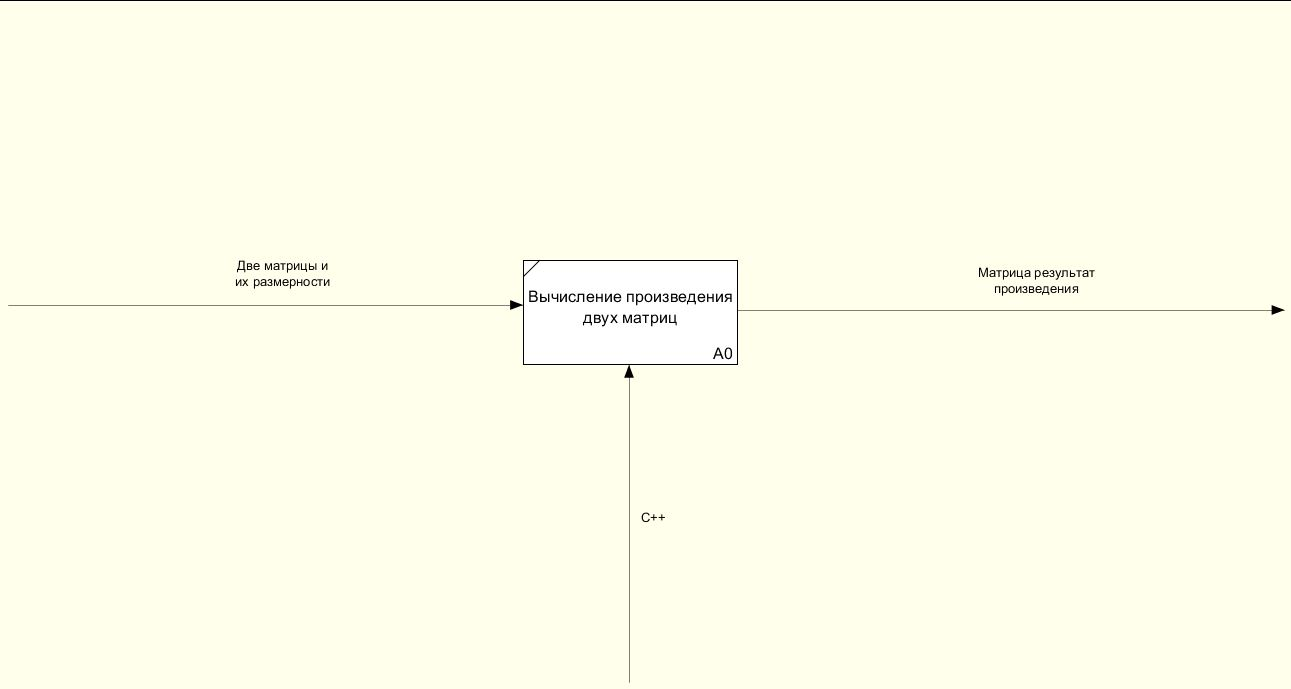
\includegraphics[width=1\linewidth]{idef.jpg}
\caption{IDEF0-диаграмма, описывающая алгоритм сортировка массива}
\label{fig:mpr}
\end{figure}




\begin{figure}[!ht]
\centering
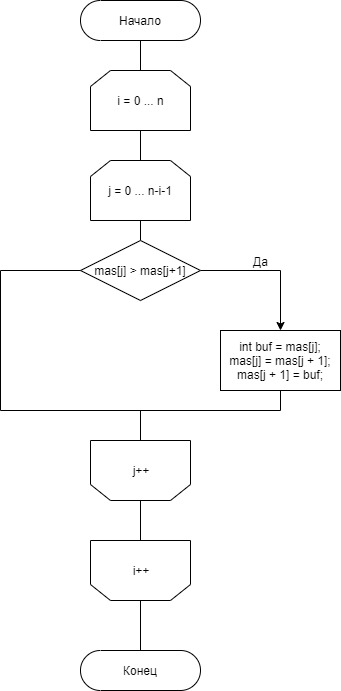
\includegraphics[width=0.6\linewidth]{diag_bubble.jpg}
\caption{Схема алгоритма сортировки "пузырьком"}
\label{fig:mpr}
\end{figure}

\begin{figure}[h]
\centering
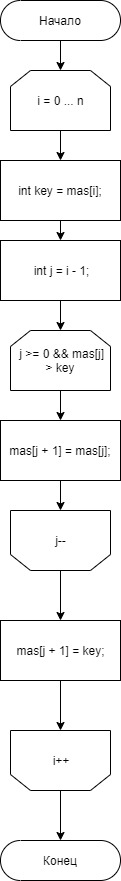
\includegraphics[scale=0.6]{diag_inst.jpg}
\caption{Схема алгоритма сортировки "вставками"}
\label{fig:mpr}
\end{figure}

\begin{figure}[h]
\centering
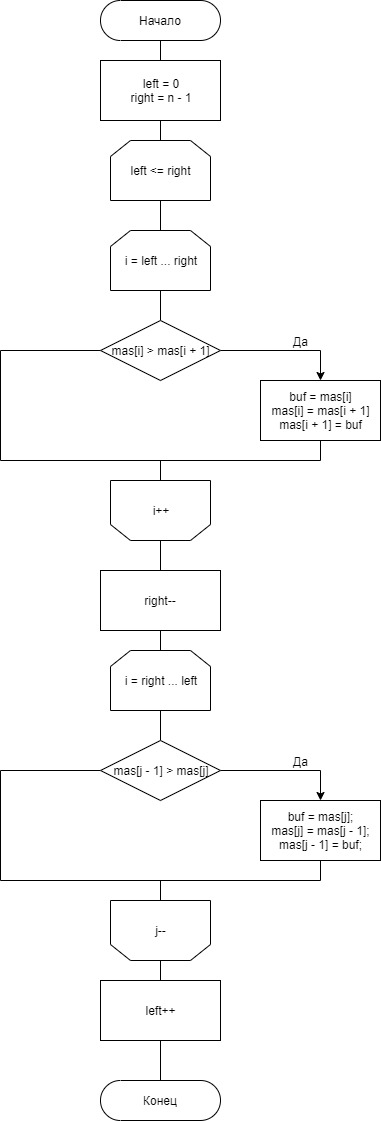
\includegraphics[scale=0.45]{diag_shaker.jpg}
\caption{Схема алгоритма шейкерной сортировки}
\label{fig:mpr}
\end{figure}

\section{Трудоемкость алгоритмов}
Введем модель трудоемкости для оценки алгоритмов: 
\begin{itemize}
	\item базовые операции стоимостью 1 — +, -, *, /, =, ==, <=, >=, !=, +=, []
	\item оценка трудоемкости цикла for от 0 до N с шагом 1 $F_{for} = 2 + N \cdot (2 + F_{body})$, где $F_{body}$ - тело цикла
	\item стоимость условного перехода применим за 0, стоимость вычисления условия остаётся
\end{itemize}

Оценим трудоемкость алгоритмов по коду программы

\subsection{Сортировка пузырьком}
Рассмотрим трудоемкость сортировки пузырьком:\\

Лучший случай: $2 + 2N + 3NN$ \\

Худший случай: $2 + 2N + 6NN$



\subsection{Сортировка вставками}

Рассмотрим трудоемкость сортировки вставками:\\

Лучший случай: $2 + 9N + 7/2NN$ \\

Худший случай: $2 + 2N + 11/2NN$


\subsection{Шейкерная сортировка}

Рассмотрим трудоемкость шейкерной сортировки:\\


Лучший случай: $12NN + 7N + 5$ \\

Худший случай: $28NN + 7N + 5$

\section{Схемы алгоритмов}
В данной части будут рассмотрены схемы алгоритмов. \\
На рис. 2.2 представлена  схема алгоритма сортировки "пузырьком".\\
На рис. 2.3 представлена  схема алгоритма сортировки "вставками".\\
На рис. 2.4 представлена  схема алгоритма шейкерной сортировки.\\



\chapter{Технологическая часть}
\section{Выбор ЯП}
Для реализации программ я выбрала язык программирования C++, так имею большой опыт работы с ним. Среда разработки - Visual Studio. \\

Для замера процессорного времени используется функция, возвращающая количество тиков.\\

\begin{lstlisting}[label=some-code,caption=Функция получения тиков]
unsigned long long getTicks(void)
{
    unsigned long long d;
    __asm__ __volatile__ ("rdtsc" : "=A" (d) );
    return d;
}

\end{lstlisting}

\section{Реализация алгоритма}

\begin{lstlisting}[label=some-code,caption=Алгоритм сортировки пузырьком]
void sortBubble(int* mas, int n) 
{ 
	for (int i = 0; i < n; i++)         
		for (int j = 0; j < n - i - 1; j++)             
			if (mas[j] > mas[j + 1])
			{
				int buf = mas[j];
				mas[j] = mas[j + 1];
				mas[j + 1] = buf;
			}
}
\end{lstlisting}


\begin{lstlisting}[label=some-code,caption=Алгоритм сортировки вставками]
void sortInsertion(int* mas, int n) 
{ 
	for (int i = 1; i < n; i++) 
	{ 
		int key = mas[i];         
		int j = i - 1;         
		for (; j >= 0 && mas[j] > key; j--)             
			mas[j + 1] = mas[j];         
		mas[j + 1] = key; 
	} 
}
\end{lstlisting}


\begin{lstlisting}[label=some-code,caption=Алгоритм шейкерной сортировки]
void sortShaker(int *mas, int n)
{
	int left = 0, right = n - 1;
	while (left <= right)
	{
		for (int i = left; i < right; i++)
		{
			if (mas[i] > mas[i + 1])
			{
				int buf = mas[i];
				mas[i] = mas[i + 1];
				mas[i + 1] = buf;
			}
		}
		right--;
		for (int j = right; j >= left; j--)
		{
			if (mas[j - 1] > mas[j])
			{
				int buf = mas[j];
				mas[j] = mas[j - 1];
				mas[j - 1] = buf;
			}
		}
		left++;
	}
}
\end{lstlisting}

\section{Тестовые данные}

Проверка работы алгоритмов на примерах:
\begin{itemize}
	\item массив, заполненные случайными числами
	\item отсортированные массивы
	\item отсортированные в обратном порядке массивы
\end{itemize}

\begin{figure}[!htbp]
\centering
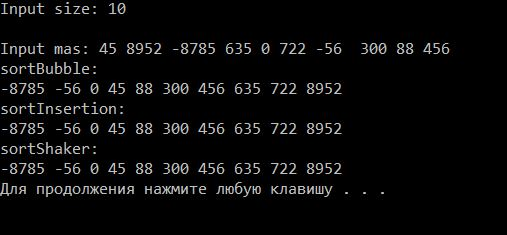
\includegraphics[width=1\linewidth]{example1.jpg}
\caption{Пример работы алгоритмов с массивом, заполненным случайными числами}
\label{fig:mpr}
\end{figure}

\begin{figure}[!htbp]
\centering
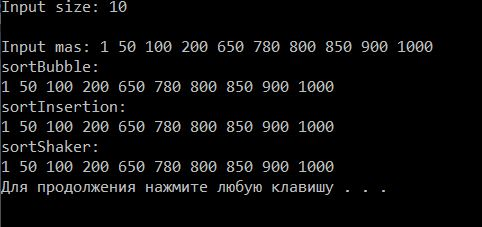
\includegraphics[width=1\linewidth]{example2.jpg}
\caption{Пример работы алгоритмов с отсортированным массивом}
\label{fig:mpr}
\end{figure}

\begin{figure}[!htbp]
\centering
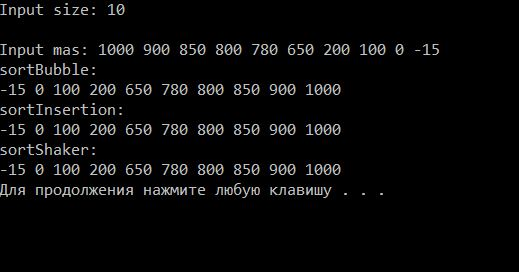
\includegraphics[width=1\linewidth]{example3.jpg}
\caption{Пример работы алгоритмов с отсортированным в обратном порядке массивом}
\label{fig:mpr}
\end{figure}




\chapter{Исследовательская часть}

\section{Сравнительный анализ на основе замеров времени работы алгоритмов}

Был проведен замер времени работы каждого из алгоритмов.\\

Сравнение времени сортировки массивов, заполненных случайными числами: \\


\begin{tikzpicture} 
\begin{axis} [
    	axis lines = left,
    	xlabel={Размер матрицы},
    	ylabel={Время (тики)},
    	xmin=100, xmax=1000,
    	ymin=0, ymax=700000,
	legend pos=north west,
	ymajorgrids=true
]
\addplot[color=red, mark=square] table[x index=0, y index=1] {Bubble.dat}; 
\addplot[color=green, mark=square] table[x index=0, y index=1] {Inst.dat};
\addplot[color=blue, mark=square] table[x index=0, y index=1] {Shaker.dat};

\addlegendentry{Пузырёк}
\addlegendentry{Вставки}
\addlegendentry{Шейкер}
\end{axis}
\end{tikzpicture}
\begin{center}
  	Рисунок 4.4. График времени работы алгоритмов сортировки массивов, заполненных случайными числами
	\end{center}
	
Сравнение времени сортировки массивов, удовлетворяющие лучшим случаям выполнения алгоритма:  \\
	
\begin{tikzpicture}
\begin{axis}[
    	axis lines = left,
    	xlabel={Размер матрицы},
    	ylabel={Время (тики)},
    	xmin=100, xmax=1000,
    	ymin=0, ymax=700000,
	legend pos=north west,
	ymajorgrids=true
]
\addplot[color=red, mark=square] table[x index=0, y index=1] {Bubble_1.dat}; 
\addplot[color=green, mark=square] table[x index=0, y index=1] {Inst_1.dat};
\addplot[color=blue, mark=square] table[x index=0, y index=1] {Shaker_1.dat};

\addlegendentry{Пузырёк}
\addlegendentry{Вставки}
\addlegendentry{Шейкер}
\end{axis}
\end{tikzpicture}
\begin{center}
  	Рисунок 4.5. График времени работы алгоритмов сортировки массивов, удовлетворяющие лучшим случаям выполнения алгоритма
	\end{center}
	
Сравнение времени сортировки массивов, удовлетворяющие худшим  случаям выполнения алгоритма: \\
	
\begin{tikzpicture}
\begin{axis}[
    	axis lines = left,
    	xlabel={Размер матрицы},
    	ylabel={Время (тики)},
    	xmin=100, xmax=1000,
    	ymin=0, ymax=700000,
	legend pos=north west,
	ymajorgrids=true
]
\addplot[color=red, mark=square] table[x index=0, y index=1] {Bubble_2.dat}; 
\addplot[color=green, mark=square] table[x index=0, y index=1] {Inst_2.dat};
\addplot[color=blue, mark=square] table[x index=0, y index=1] {Shaker_2.dat};

\addlegendentry{Пузырёк}
\addlegendentry{Вставки}
\addlegendentry{Шейкер}
\end{axis}
\end{tikzpicture}
\begin{center}
  	Рисунок 4.6. График времени работы алгоритмов сортировки массивов, удовлетворяющие худшим случаям выполнения алгоритма
	\end{center}
	
\subsection{Вывод}
По результатам тестирования выявлено, что все рассматриваемые алгоритмы реализованы правильно. Самым быстрым алгоритмом, при использовании случайного заполнения, оказался алгоритм сортировки «вставками», а алгоритмы сортировки «пузырьком» и «шейкер» являются разновидностями пузырьковой сортировки, их результаты схожи, однако на массивах большей длины выигрывает классическая сортировка «пузырьком». 




\chapter*{Заключение}
\addcontentsline{toc}{chapter}{Заключение}
В ходе работы были изучены алгоритмы сортировки массива: «пузырек», «вставки» и «шейкер». Выполнено сравнение всех рассматриваемых алгоритмов. Изучены зависимости выполнения алгоритмов от длины массива. Также реализован программный код продукта


\end{document}